\chapter{Vergleich der beiden Algorithmen}

Beim Betrachten der beiden Algorithmen f�llt auf,
dass Worst- und Best-Case Situationen absolut identische Effizienzgrade haben.\\
Der Best-Case ist nat�rlich der Fall, in dem direkt in der ersten Iteration das Ziel gefunden wurde.\\
Der Worst-Case dem entsprechend, wenn das Ziel nicht zu finden, oder der letzte erreichbare Knoten ist.\\
Das zeigt, dass die Verbesserungen, welche A* von Dijkstras Algorithmus unterscheiden, nur ins Auge springen, wenn die Wegkosten gesch�tzt werden k�nnen.
Ein offenes Feld mit diversen, einfachen Hindernissen ist demnach mehr geeignet als ein Labyrinth, welches nur wenige Strecken zum Ausgang zul�sst.\\
\newpage
Wie auf \ref{DvsA} zu sehen, kann eine gleiche Ausgangssituation unterschiedlich schnell gel�st werden. Da Dijkstra keine Pr�ferenzen beim W�hlen der Knoten hat, sucht er alle Kanten, unabh�ngig von der Entfernung, ab. \\
A* hingegen besucht deutlich weniger Knoten. In dieser Situation lief er zuerst in das Hindernis. Verhielt sich anschlie�end wie Dijkstra, bis ein Weg um das Hindernis gefunden wurde. Wie in \ref{lastFrameA} und \ref{lastFrameD} zu sehen.


\begin{figure}
\centering
\caption{Dikstra Vergleich A*}
\label{DvsA}
%\caption{Dikstra Vergleich A*}
\begin{subfigure}[b]{0.5\textwidth} %[hbtp]
	\centering
		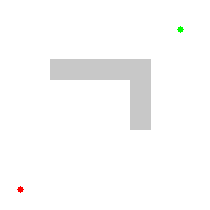
\includegraphics[width=\textwidth]{images/progress_Path_animation_firstframe.png}
	\caption{Ausganssituation}
	\label{Frame1}

\end{subfigure}
\\
\begin{subfigure}[b]{0.49\textwidth} %[hbtp]
	\centering
		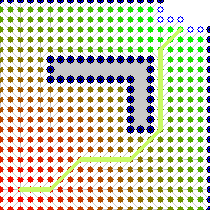
\includegraphics[width=\textwidth]{images/progress_Dijkstras_animation_lastframe.png}
	\caption{Endsituation Dijkstra}
		\label{lastFrameD}
\end{subfigure}
\begin{subfigure}[b]{0.49\textwidth} %[hbtp]
	\centering
		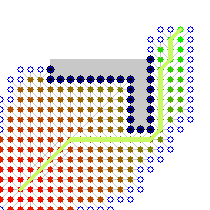
\includegraphics[width=\textwidth]{images/progress_Astar_animation_lastframe.png}
	\caption{Endsituation A*}
		\label{lastFrameA}
\end{subfigure}
{\small{\it{Quelle: http://upload.wikimedia.org/wikipedia/commons/5/5d/Astar\_progress\_animation.gif}}}\\
{\small{\it{Quelle: http://upload.wikimedia.org/wikipedia/commons/2/23/Dijkstras\_progress\_animation.gif}}}
\end{figure}
